% +--------------------------------------------------------------------+
% | Sample Chapter 4
% +--------------------------------------------------------------------+

\cleardoublepage

% +--------------------------------------------------------------------+
% | Replace "This is Chapter 4" below with the title of your chapter.
% | LaTeX will automatically number the chapters.
% +--------------------------------------------------------------------+

\chapter{Implementación}
\label{makereference4}
Nuestra aplicación es una aplicación móvil desarrollada en Android, Unity y Vuforia y con un servidor desarrollado en Java usando Spring.
En este capítulo comenzaremos mostrando todos los prototipos de implementación que hemos desarrollado, en los cuáles veremos los pros y contras de las
tecnologías que hemos probado y el porqué de nuestra elección de implementar la aplicación con estas tecnologías. 
Después describiremos cómo hemos implementado nuestra aplicación, desde la arquitectura que hemos seguido, 
las tecnologías usadas para la parte frontend y la parte backend junto a las dificultades 
que nos hemos encontrado mientras trabajábamos. Finalmente hablaremos de las herramientas de trabajo
utilizadas para facilitarnos el trabajo en equipo.
\section{Prototipos}
\label{makereference4.1}

\subsection{ARCore} 
\label{makereference4.1.1} 
    Al comenzar la fase de desarrollo de proyectos, pensamos que una de las tecnologías que debíamos 
    investigar y probar debía ser ARCore. Esto se debía a que, la empresa detrás de esta 
    tecnología es Google y esto podría significar que tendríamos más material de consulta 
    y ejemplos en comparación con otras tecnologías de fabricantes con menos recursos.
    ARCore se encuentra disponible para Java, Unity, Unreal e iOS. Comenzamos realizando el 
    "Quickstart"\ para Android y posteriormente para Unity. 
    Tras realizar los proyectos propuestos por ARCore, realizamos algún proyecto propio 
    para comprobar si la herramienta se ajustaba a la idea que teníamos para nuestro futuro proyecto.
    Tras realizar ambos proyectos, concluimos que, aunque ARCore reúne las características 
    necesarias para en un futuro convertirse en una de las tecnologías más importantes en Realidad Aumentada, 
    no íbamos a seleccionarla para nuestro proyecto por las siguientes razones:
    \begin{itemize}
        \item Dispone de mucha documentación para comenzar a usar la herramienta, pero poca para realizar tareas más complejas.
        \item Resulta muy útil para realizar superposiciones de modelos 3D sobre superficies. Sin embargo, una de las funcionalidades más importantes que nuestra aplicación requería era la interacción con la realidad aumentada mediante el uso de botones, imágenes y la carga dinámica de elementos para posicionar en la pantalla de Realidad Aumentada e interaccionar con el usuario. En este sentido ARCore no está, por el momento, tan preparada como otras tecnologías.
    \end{itemize}
\subsection{Viro Media} 
\label{makereference4.1.2}

El objetivo del prototipo realizado con Viro Media es reconocer imágenes almacenadas en el dispositivo para mostrar texto y
objetos virtuales. Además de probar tecnologías de desarrollo móvil web como en este caso React Native
para plataformas iOS y Android. Comenzamos construyendo una interfaz sencilla con botones que nos redirigen a la escena de Realidad Aumentada, ver Figura \ref{fig:nativeBase_android} y \ref{fig:nativeBase_ios}.
Para esta interfaz utilizamos NativeBase que es una librería que nos permite
realizar una aplicación con apariencias de tipo iOS o Android según el dispositivo.

\begin{figure}[htb]
    \centering
    \makebox[0pt][c]{%
    \begin{minipage}[b]{0.5\linewidth}
    \centering
      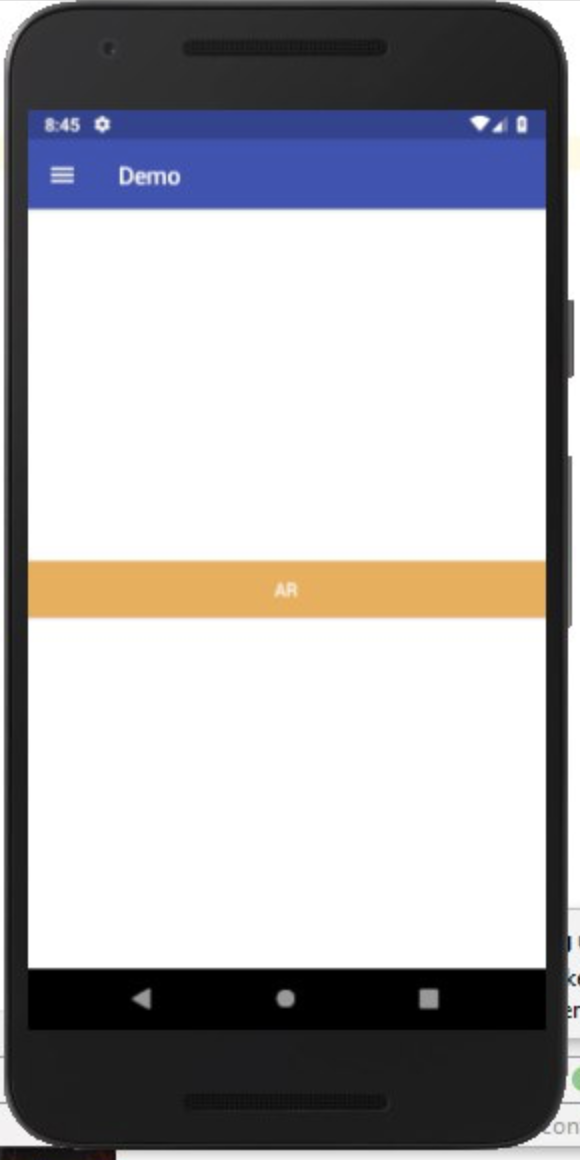
\includegraphics[scale=0.3]{figures/chapter-3/viromedia/android.png}
      \caption{Visualización con NativeBase en Android}
    \label{fig:nativeBase_android}
    \end{minipage}%
    \hspace{0.3cm}
    \begin{minipage}[b]{0.5\linewidth}
    \centering
     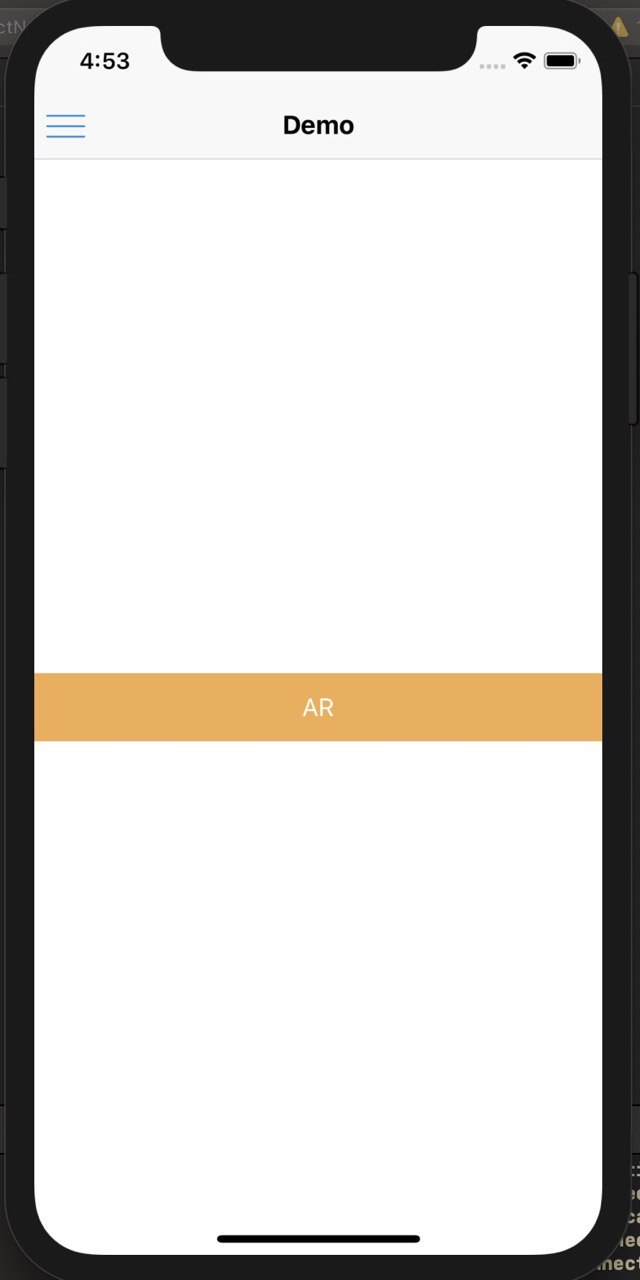
\includegraphics[scale=0.3]{figures/chapter-3/viromedia/ios.jpg}
      \caption{Visualización con NativeBase en iOS}
    \label{fig:nativeBase_ios}
    \end{minipage}%
    }%
\end{figure}

Para la escena de realidad aumentada mostramos texto y al detectar el póster de Pantera Negra,
reacciona mostrando una animación de dicho superhéroe saliendo del póster, ver Figura \ref{fig:visualizacionRANAtibe}.
 
\begin{figure}[H]
    \centering
    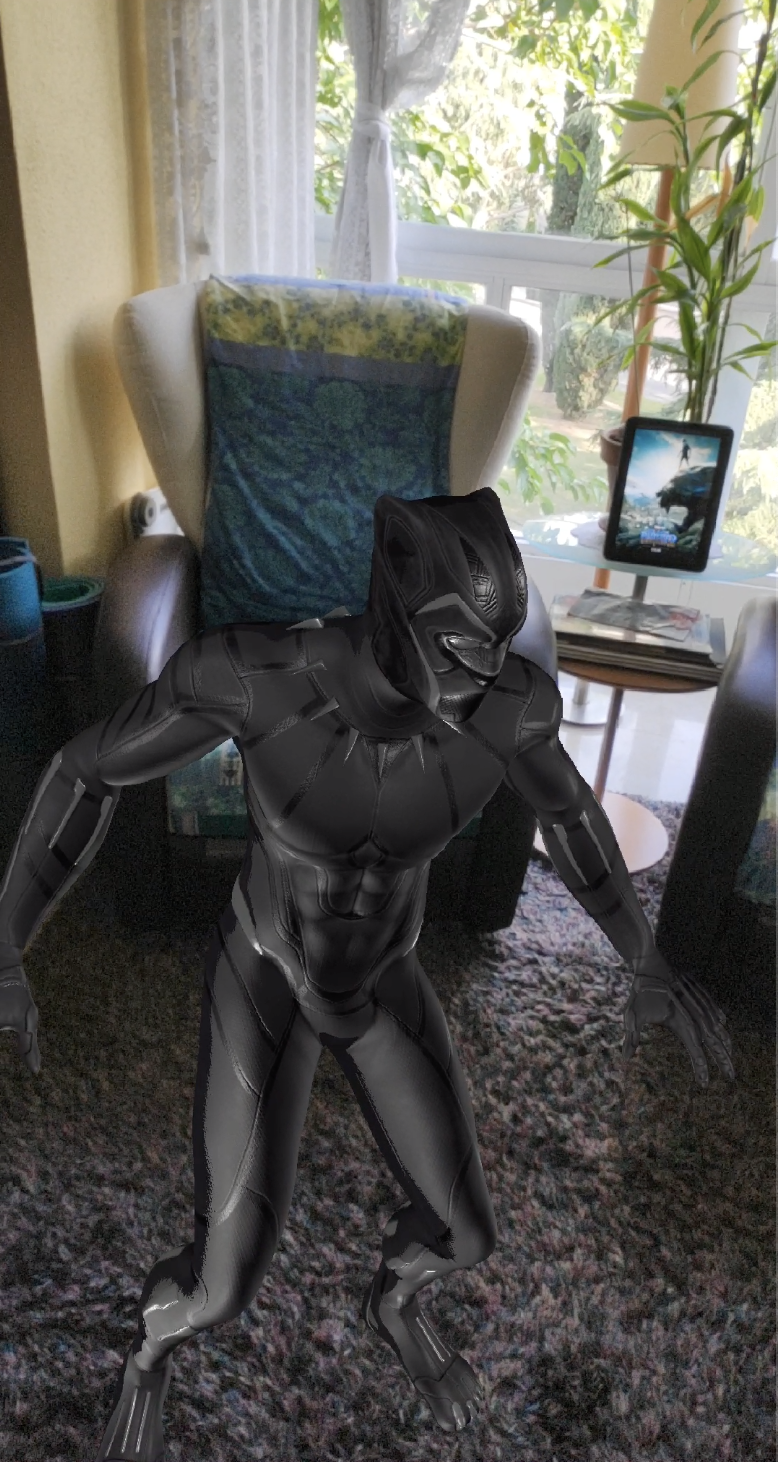
\includegraphics[height=4in]{figures/chapter-3/viromedia/blackpanther.png}
    \caption{Visualización de RA}
    \label{fig:visualizacionRANAtibe}
\end{figure}
\newpage
Una de las ventajas que apreciamos fue la facilidad del lenguaje, en este caso Javascript,
 utilizando la popular librería ReactJS y la buena documentación de Viro Media
 que hacían que el proceso de codificación fuera agradable.\\

Uno de los problemas que presentaba este prototipo era que las dependencias de Viro Media entraban en conflicto con las de NativeBase
imposibilitándonos la forma de encontrar versiones compatibles. Utilizamos las últimas que, a pesar de lanzar
 advertencias, funcionaba en el ejemplo realizado.
Otro problema fue la compilación de la aplicación, Viro Media tiene una aplicación para probar lo
 que desarrollamos conectándose a nuestro ordenador a través de la red. El problema es
 que algunos recursos, como los iconos que utilizaba NativeBase, no eran descargados, por lo que la
 mejor forma era probar la versión compilada de iOS y Android. La forma de compilar
 la aplicación era un proceso costoso para los ordenadores, lento y con multitud de problemas según
 se ampliaban las librerías que se utilizan.\\

La conclusión que obtuvimos de este prototipo fue que Viro Media y React Native son tecnologías muy prometedoras, pero debido a los
 problemas surgidos y a que todas sus versiones no eran estables vimos un claro riesgo para

\subsection{Vuforia + Android} 
\label{makereference4.1.3} 
 
En este prototipo utilizamos la librería nativa de Vuforia para Android para 
realizar las pruebas de tecnología de reconocimiento de imágenes tanto en  
local como usando la nube que nos ofrecía Vuforia, para la posterior renderización
de objetos y textos.

Las características tecnológicas de este prototipo son las siguientes:


\begin{enumerate}
    \item La librería de Vuforia para Android está diseñada a muy bajo nivel.
    \item Vuforia para dibujar en 3D usa la librería OpenGL, ver Figura \ref{fig:modelo3D}.
    \item OpenGL utiliza una serie de espacios donde se van colocando los elementos, ver Figura \ref{fig:esquemaOpenGl}: 
    \begin{enumerate}
        \item Local space: Es el espacio local de cada objeto.
        \item World space: Es el mundo donde se encuentran los objetos.
        \item View space: El mundo visto desde la perspectiva de la cámara.
        \item Clip space: Se integra con la pantalla del móvil y, definiendo los límites visibles, se establecen unas coordenadas de rango (-1,-1) - (1,1).
    \end{enumerate}
    
        Las transformaciones de estos espacios se realizan mediante matrices 4x4, 
        en las que la primera fila hace referencia a la coordenada $x$, la segunda a la coordenada $y$ y la 
        tercera a la coordenada $z$, mientras que la última columna hace referencia a los desplazamientos 
        de los objetos en esos 3 ejes.
            \begin{figure}[H]
                \centering
                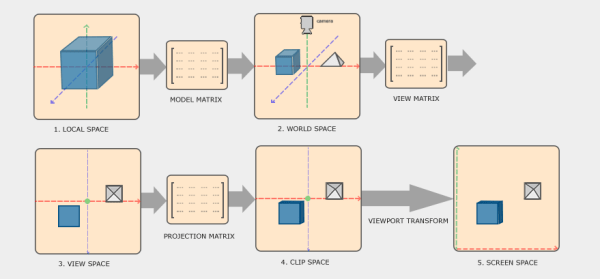
\includegraphics[width=5in]{figures/space-transformation.png}
                \caption{Esquema de los distintos espacios que usa OpenGL\cite{spaceopengl}}
                \label{fig:esquemaOpenGl}
            \end{figure}


            \begin{figure}[H]
                \centering
                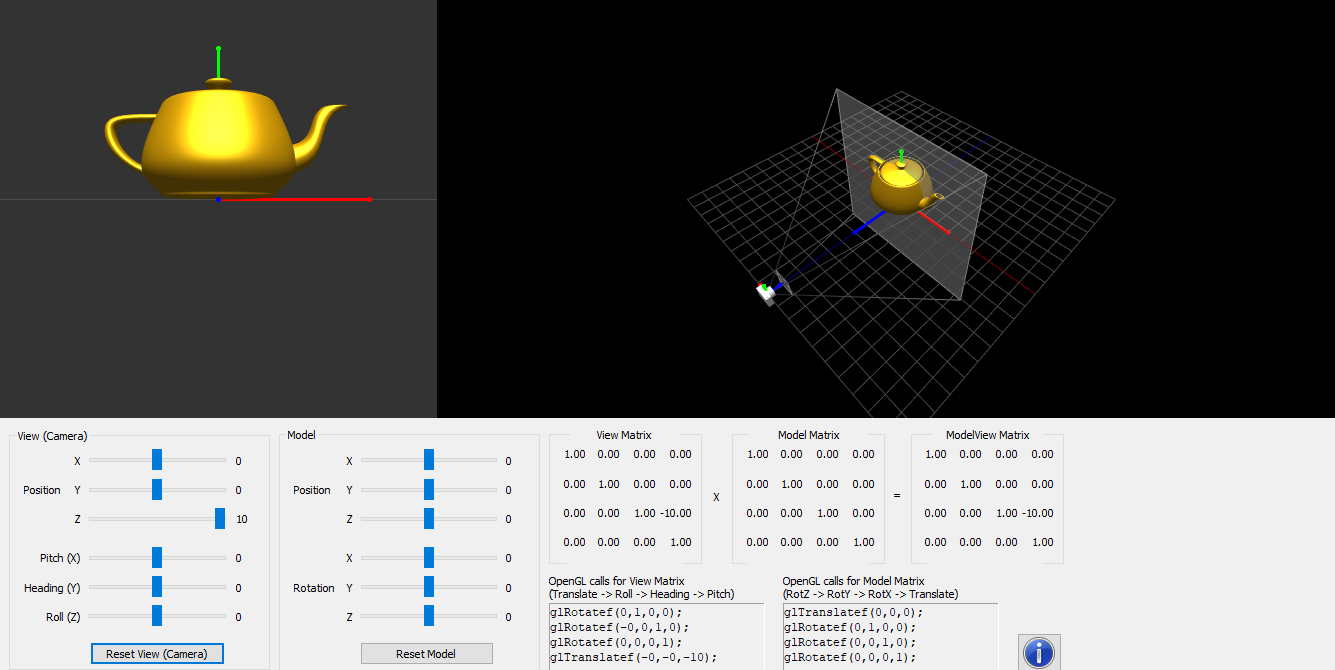
\includegraphics[width=5in]{figures/teapot.png}
                \caption{Captura de un ejemplo de un modelo en 3D}
                \label{fig:modelo3D}
            \end{figure}

    
    \item En OpenGL es necesario escribir código para que las tarjetas gráficas rendericen el modelo 3D,
    el lenguaje que se usa es GLSL. Este código de GLSL se escribe en forma de String y se llama a un método 
    que proporciona OpenGL, podemos ver un ejemplo de este código en la Figura \ref{fig:codigoGLSL}.
    \begin{figure}[H]
        \centering
        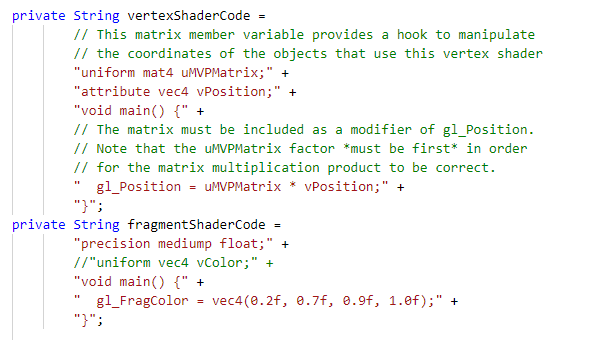
\includegraphics[width=5in]{figures/GLSL.png}
        \caption{Código en GLSL}
        \label{fig:codigoGLSL}
    \end{figure}
    \newpage    
    \item Otro aspecto a tener en cuenta es que OpenGL solo nos ofrece lo básico, no nos ofrece métodos para dibujar 
    directamente objetos, sino que hay que seguir un pipeline de procesos para conseguir dibujar algo, ver Figura \ref{fig:pipeline}.
    Esto consiste en pasar un array de números (cada tres para definir un punto) 
    a las tarjetas gráficas, establecer triángulos entre los puntos (más arrays de números) 
    definir colores a partir de los puntos (más arrays...), y con el código del shader, ejecutar 
    estos datos.
    \begin{figure}
        \centering
        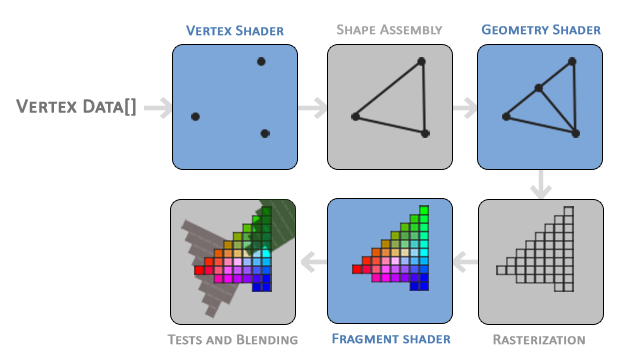
\includegraphics[width=4in]{figures/pipeline.png}
        \caption{Pipeline de la construcción de un modelo\cite{pipelineopengl}}
        \label{fig:pipeline}
    \end{figure}
    \item Por último, como sólo ofrece métodos básicos, no hay métodos de escritura de texto, y la forma que 
    encontramos para que funcione fue usar un bitmap con los caracteres, ver Figura \ref{fig:mapaBits}.Este fue el principal 
    motivo de rechazar esta tecnología ya que, dependiendo de la funcionalidad que se desee implementar, es necesario codificar a muy bajo nivel, lo que costaría mucho tiempo y esfuerzo.
    \begin{figure}
        \centering
        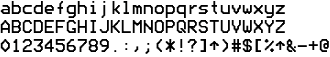
\includegraphics[width=5in]{figures/bitmap-font.png}
        \caption{Mapa de bits de caracteres usado}
        \label{fig:mapaBits}
    \end{figure}
\end{enumerate}

\subsection{Vuforia + Unity} 
\label{makereference4.1.4}

    Para realizar este prototipo utilizamos Unity como herramienta básica para realizar la aplicación y Vuforia para dar soporte a la realidad aumentada.
    El prototipo a desarrollar consistió en un modelo 3D de un dragón que aparecía al detectar una imagen que previamente habíamos establecido como ``imagen objetivo''.

    \begin{figure}[H]
        \centering
        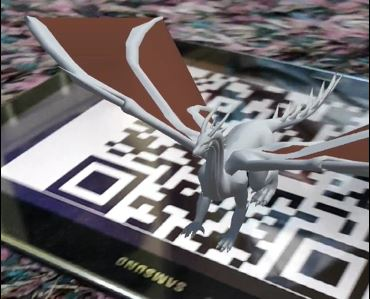
\includegraphics[width=5in]{figures/prototipoUnity.jpg}
        \caption{Modelo en 3D que aparecía al detectar la imagen}
    \end{figure}

Pese a que nadie del equipo había utilizado Unity previamente el resultado fue bastante positivo ya que:
\begin{enumerate}
    \item Unity resultó ser intuitivo y relativamente fácil en cuanto al aprendizaje de las funcionalidades básicas.
    \item Vuforia parecía estar muy probada e incluía de serie muchas funcionalidades.
    \item Vuforia tenía la opción de utilizar un Cloud para almacenar las imágenes objetivo.
\end{enumerate}


\subsection{Vuforia + Unity + Android} 
\label{makereference4.1.5}

Una vez realizado el prototipo en Vuforia con Unity comenzamos a investigar cómo realizar el resto de la aplicación que no requería de Realidad Aumentada.
Hasta este momento teníamos claro que Vuforia con Unity era la mejor combinación para realizar la parte de realidad aumentada. Sin embargo, tras realizar pruebas desarrollando en Unity interfaces y lógica nos dimos cuenta de que Unity no era igual de intuitivo ni eficaz a la hora de realizar estas tareas que necesitábamos para desarrollar el resto de la aplicación que no necesitaba Realidad Aumentada.
Por este motivo intentamos buscar la opción de realizar una aplicación en la que la realidad aumentada estuviese diseñada en Unity con Vuforia y el resto de la aplicación en Android, ver Figura \ref{fig:botonAndroidUnity}.

\begin{figure}[H]
    \centering
    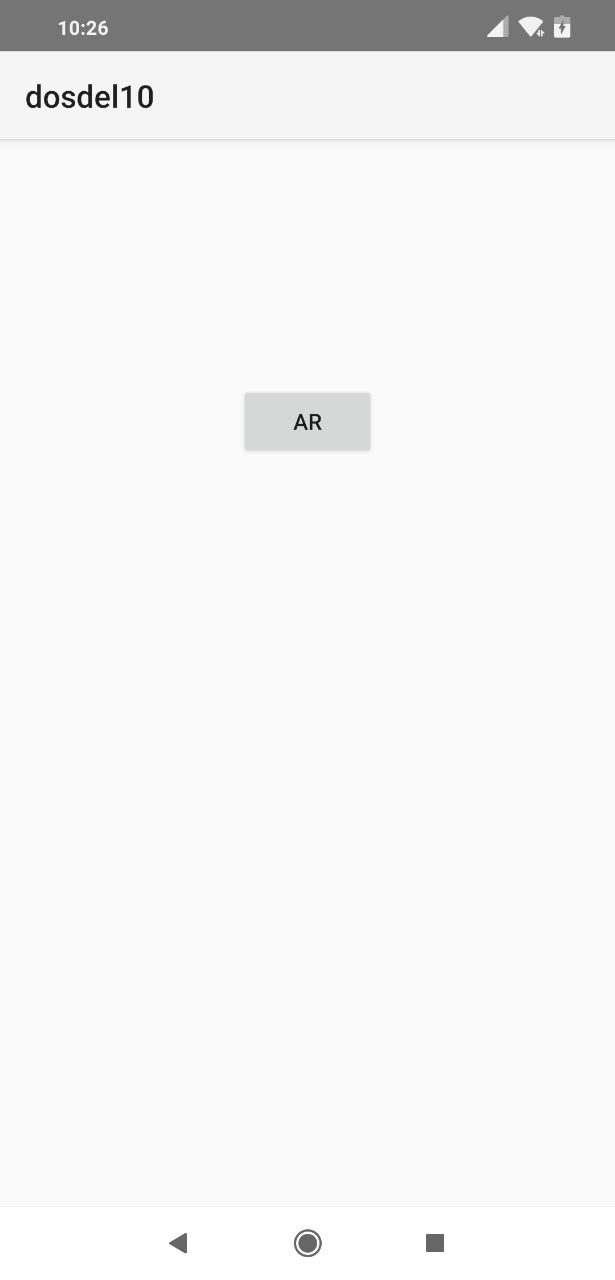
\includegraphics[height=4in]{figures/androidUnityVuforia.jpg}
    \caption{Botón que comunica Android con Unity}
    \label{fig:botonAndroidUnity}
\end{figure}

Finalmente conseguimos tener ambos proyectos independientes. La realidad aumentada se desarrollaba en Unity con Vuforia y se exportaba a un proyecto Android donde se encontraba el resto de la aplicación.
Esto nos permitía realizar la realidad aumentada con la herramienta que tras las primeras tomas de contacto habíamos comprobado que era la mejor (Unity con Vuforia) y del mismo modo realizar el resto de la aplicación con la mejor herramienta para esta parte (Android Studio).

Tras realizar este prototipo, consideramos que estas herramientas podrían ser las que usásemos en la aplicación final puesto que:
\begin{enumerate}
    \item Como ya habíamos descubierto en el prototipo anterior, Unity era una herramienta muy completa y junto con Vuforia nos proporcionaban todas las herramientas necesarias para cumplir con los casos de uso de Realidad Aumentada que teníamos en mente.
    \item Al haber encontrado la forma de combinar Unity y Android no teníamos que renunciar a ninguna de las dos herramientas. Lo que nos permitía explotar las cosas buenas de ambas herramientas.
    \item La comunicación entre Unity y Android era relativamente sencilla pese a ser dos proyectos distintos.
\end{enumerate}


\subsection{Server en Spring} 
\label{makereference4.1.6}

Para la realización de la parte backend de la aplicación decidimos
incorporar la tecnología de Spring para codificar un servicio web REST en Java
y el acceso a datos mediante MySQL. Para el prototipo seguimos un tutorial\cite{tutorialspring} de 3 partes para crear un servicio web REST
que gestionara una simple entidad de contactos de personas, con atributos como el nombre completo del contacto, su número de teléfono o su correo electrónico. Se puede observar su estructura
en la figura \ref{fig:entidadContactos}.
    \begin{figure}[H]
        \centering
        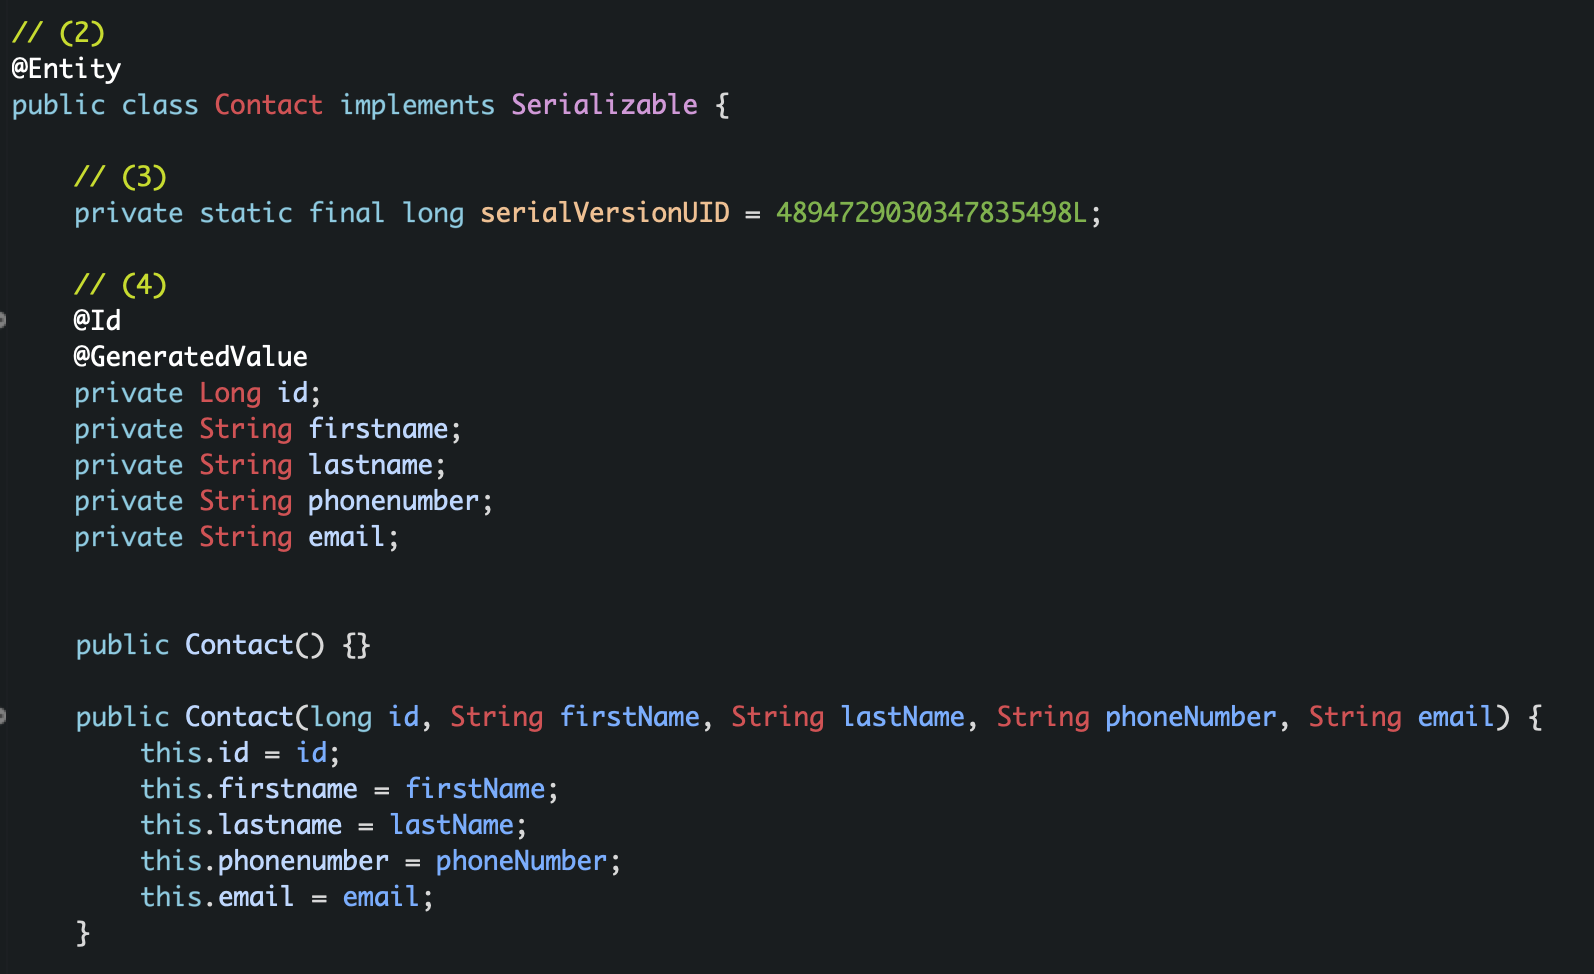
\includegraphics[width=6in]{figures/ContactsEntity.png}
        \caption{Entidad de Contactos}
        \label{fig:entidadContactos}
    \end{figure}

También se investigaron distintas formas de realizar el acceso a la base de datos desde el servidor, nos decantamos por una clase que nos ofrecía implementados los métodos básicos para crear, leer, actualizar y borrar datos. Además de la opción 
de poder crear nuestros propios métodos.

Para este prototipo decidimos usar MySQL como sistema de gestión de bases de datos relacional, aunque
a la hora de probar a levantar nuestro servidor de prueba tuvimos que rehacer este prototipo, además de adaptarlo para 
que gestionara entidades de películas, y que usara PostgreSQL.
\section{Arquitectura}
\label{makereference4.2}
En cuanto a la arquitectura usada en nuestra aplicación hemos adjuntado un esquema que podemos observar en la Figura \ref{fig:arquitectura}. Nuestra aplicación móvil estará implementada tanto en Android
como en Unity, la aplicación general está en Android, mientras que la parte de realidad aumentada está desarrollada en Unity y usa Vuforia. Para el reconocimiento
de imágenes con Vuforia usamos un almacenamiento en la nube gratuito que nos ofrece para almacenar las imágenes ya que, tener todas las imágenes en la misma aplicación la cargaría de un peso innecesario. Vuforia es una herramienta de pago, sin embargo, 
ofrece una licencia gratuita para desarrolladores que pretendan aprender la tecnología sin lucrarse de ella\cite{vuforia_prices}. Tiene limitaciones como el número de accesos al mes o el número de imágenes que se pueden guardar, pero para el uso que pretendemos 
darle es suficiente \cite{vuforia_free}. 
Para la parte del servidor, hemos realizado una API Rest con Spring, usando además una base de datos relacional en PostgreSQL. La comunicación entre cliente y servidor se realiza mediante peticiones HTTP a 
nuestro servidor desplegado en Heroku el cual nos devolverá los datos en formato JSON y posteriormente los mapearemos a una clase Java.
\begin{figure}[H]
    \centering
    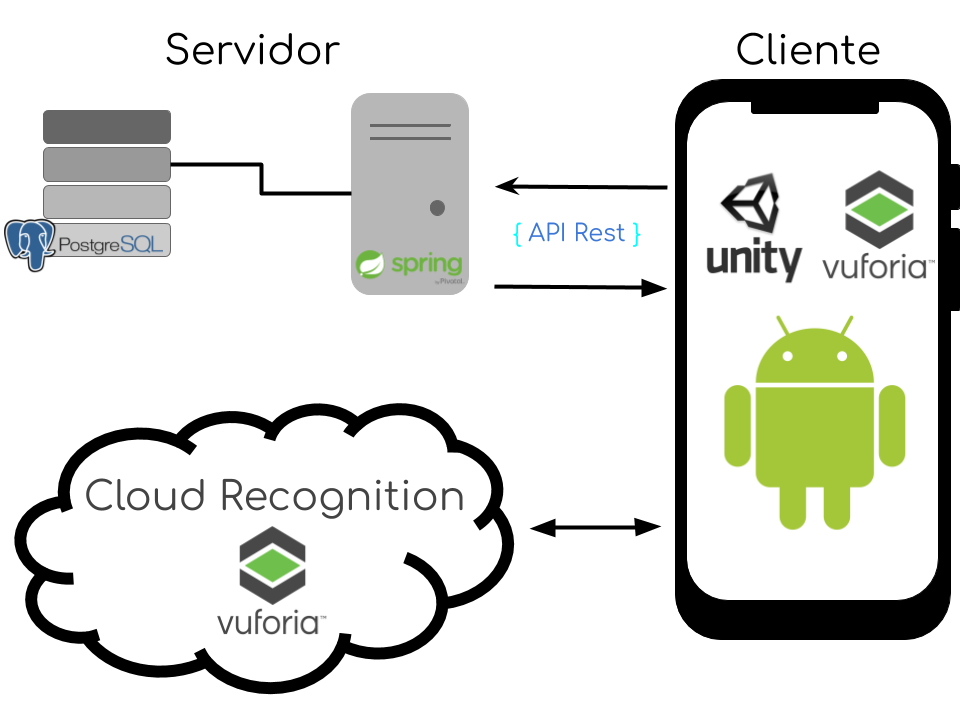
\includegraphics[width=6in]{figures/chapter-4/arquitectura.png}
    \caption{Arquitectura}
    \label{fig:arquitectura}
\end{figure}
\section{Servidor}
\label{makereference4.3}
Nuestro servidor está programado en Java, usando el framework Spring para la creación de una API Rest que mediante peticiones HTTP y una base de datos relacional en PostgreSQL nos proporcionará
toda la información necesaria para alimentar de datos a nuestro cliente. El servidor necesita ser desplegado para que la aplicación pueda tener un uso real por lo que conseguimos desplegarlo de forma gratuita en Heroku, que además ofrece
facilidades para desplegar un servidor creado mediante Spring, por lo que nos facilitó el trabajo considerablemente. También se encuentra en el servidor la implementación del sistema de recomendación.
En el servidor tendremos todas las entidades que necesitamos representadas mediante clases Java y anotaciones de JPA, para facilitar el mapeo entre tablas de la base de datos y dichas entidades. Hemos implementado las siguientes entidades:
\begin{itemize}
    \item Film: entidad referente a las películas que guardamos, con su respectivo título, director, duración, valoración, url del trailer, sinopsis, url de la imagen de la película, género, país y fecha de estreno.
    \item User: entidad para representar a los usuarios de la aplicación, con su nombre, foto, email y contraseña.
    \item Friendship: entidad para representar la relación de amistad entre usuarios.
    \item Plan: entidad para representar los planes, estos poseerán una película, un usuario creador, fecha, hora, lugar, título, descripción y una lista de usuarios unidos.
    \item UserFilm: entidad intermedia para representar la relación de usuarios con películas, es decir, las películas que son guardadas por cierto usuario.
    \item Recommendation: entidad para representar las recomendaciones a los usuarios.
\end{itemize}
Para cada una de estas entidades necesitamos una clase Controller, que actuará de controlador para saber redirigir cada petición HTTP a su correspondiente servicio de aplicación, donde se aplicará la lógica del negocio, comprobando 
que los datos son correctos y obteniendo, modificando o creando elementos en la base de datos a través de las clases Repository correspondiente a cada entidad.
Las distintas peticiones HTTP que realizamos son las siguientes:
\begin{itemize}
    \item Film: todas las peticiones HTTP realizadas comenzarán por la url \textbf{/films} 
    \begin{itemize}
        \item Obtener todas las películas: petición de tipo GET a la url \textbf{/}.
        \item Guardar una película: petición de tipo POST con la información de la película en el body de la petición a la url \textbf{/}.
        \item Actualizar una película: petición de tipo PUT con la información de la película en el body de la petición a la url \textbf{/}.
        \item Buscar una película por su nombre: petición de tipo GET con el nombre de la película en la url \textbf{/search/name}. 
        \item Buscar una película por su id: petición de tipo GET con el id de la película en la url \textbf{/id}.
        \item Buscar una película por su uuid: petición de tipo GET con el uuid de la película en la url \textbf{/uuid/uuid}, el segundo uuid se refiere al uuid de la película que se quiera buscar.
        \item Borrar una película: petición de tipo DELETE con el id de la película en la url \textbf{/id}.
    \end{itemize}
\end{itemize}

\section{Cliente}
\label{makereference4.4}
Nuestra aplicación está implementada principalmente en Android, las interfaces principales para el uso de los planes, recomendaciones y acceso a la información de las películas guardadas han sido desarrolladas mediante Android Studio. Sin embargo,
la parte del cliente que otorga el gran valor a nuestra aplicación está desarrollada en Unity y el uso de Vuforia, todas las escenas que aparecen al reconocer carteles de películas e imágenes de usuarios fueron implementadas de esta forma. Vuforia además nos ofrece un
servicio de Cloud para el almacenamiento de imágenes, a las cuales les asocia una valoración según lo fácil que le resultará a la aplicación reconocerla y un identificador único (UUID), que es el que usaremos para guardar la distinta información de dicha película o usuario en la base de datos.
La parte de la aplicación realizada en Unity, utiliza una serie de clases de la parte desarrollada en Android para realizar las peticiones al servidor y así poder mostrar información específica cuando se reconoce una cierta imagen.
Al principio hicimos que las dos partes realizaran las peticiones en sus respectivos lenguajes, pero decidimos que sería mejor que el acceso a la capa de datos se realizara por el mismo sitio y así conseguir que las distintas capas estuvieran separadas.
Además, en un principio, las imágenes que mostramos en la parte de Android se almacenan en Google Drive y mediante la librería de Picasso las obtenemos en tiempo de ejecución, esto se ha implementado de esta forma por la misma razón por la que tenemos las imágenes a reconocer en un Cloud.
Finalmente, debido al coste en tiempo de esta operación y tras debatirlo con nuestros directores del Trabajo de Fin de Grado, hemos decidido guardar dichas imágenes en el mismo servidor para su rápida obtención.


Como la mayor parte de la aplicación está implementada en Android Studio, la estructura de ésta se adapta a lo que ofrece el IDE, consistiendo en el flujo de unas actividades y fragmentos que explicaremos a continuación.


\subsection{Actividades}
\label{makereference4.4.1}
Son los componentes de la aplicación que representan una pantalla con la que los usuarios pueden interactuar para realizar una determinada acción.

\begin{figure}[H]
    \centering
    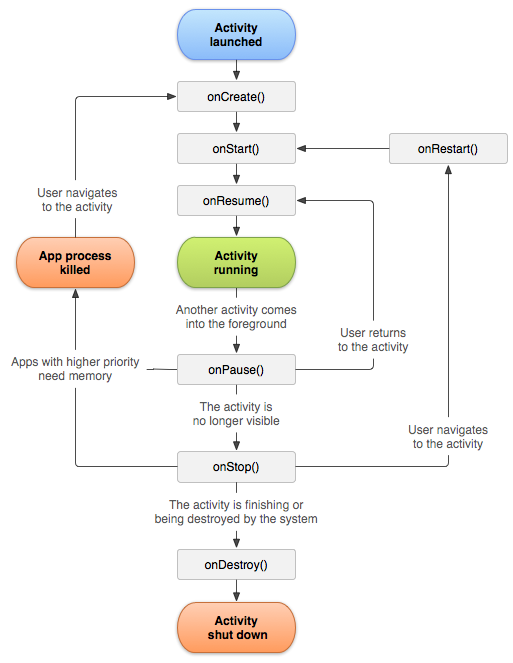
\includegraphics[width=3in]{figures/chapter-4/activity_lifecycle.png}
    \caption{Ciclo de vida de una actividad}
\end{figure}

Entre nuestras actividades podemos destacar dos: 
\begin{itemize}
    \item MainActivity: La primera actividad (actividad principal) que se activa al iniciar la aplicación, la cual comprueba el estado de sesión del usuario, si está logueado se queda en la actividad, y si no, se redirige al usuario a otra actividad llamada LoginActivity que mediante un formulario muy simple nos permite iniciar sesión o registrarnos. En MainActivity se encuentra un paginador (ViewPager) de 3 fragmentos, donde cada fragmento representa las interfaces de planes, recomendaciones y películas guardadas correspondientemente, podemos observarlo en las Figuras \ref{fig:listaPlanes}, \ref{fig:lista_peliculas} y \ref{fig:recomendaciones_1} del \autoref{makereference3}.
    \item UnityPlayerActivity: Se trata de una actividad especial que nos permite comunicar la parte desarrollada en Unity con nuestro proyecto Android. Aquí se encuentran llamadas a funciones desde la parte de Unity, se realizan las órdenes y se devuelven a Unity.
\end{itemize} 

\subsection{Adaptadores}
\label{makereference4.4.2} 
Son elementos de manipulación de datos que se aplican a vistas y componentes. En el proyecto se les ha dado mucho uso a las vistas de tipo RecyclerView para representar listas de objetos. Para manejar los datos de cada elemento de la lista, se ha utilizado un RecyclerView.Adapter, el cual manipula cada dato correspondiente a un elemento de la lista. También se han creado otros adaptadores, como uno para manejar tres fragmentos dentro de una actividad, como hemos dicho anteriormente al describir la actividad principal (MainActivity).

\subsection{Comandos}
\label{makereference4.4.3}
Aquí se encuentran todos los elementos relacionados con el patrón comando, ver Figura \ref{fig:comando}, y ha sido diseñado para realizar la conexión con la parte del proyecto desarrollado en Unity.

Este patrón permite solicitar una operación a un objeto sin conocer realmente el contenido de esta operación, ni el receptor real de la misma. Para ello se encapsula la petición como un objeto, 
lo que además facilita la parametrización de los métodos.
Lo que nos permite es abstraer la lógica de los métodos implementados en Android de Unity, es decir, si Unity necesita usarlos llamará a los comandos y esperará la respuesta.

\begin{figure}[H]
    \centering
    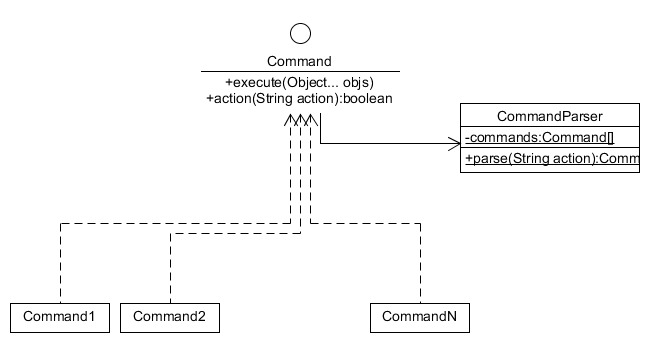
\includegraphics[width=3in]{figures/chapter-4/command_pattern.png}
    \caption{Patrón comando}
    \label{fig:comando}
\end{figure}



\subsection{Entidades}
\label{makereference4.4.4}
Todos los modelos de datos que podemos recibir del servidor, los cuales hemos descrito anteriormente en este capítulo, en la sección 4.3 describiendo el servidor, son representados por entidades en nuestro proyecto de Android, con los mismos atributos que tienen sus entidades correspondientes en el servidor.

\subsection{Fragmentos}
\label{makereference4.4.5}
Representan un comportamiento o una parte de la interfaz de usuario en una actividad.
Se utilizan para formar una vista compuesta de paginación en una actividad. 
Aquí es donde tendremos los 3 componentes principales de nuestra aplicación, la actividad referente a mis planes, la actividad de las recomendaciones y la de mis películas.

\subsection{Servicios}
\label{makereference4.4.6}
Se trata de un conjunto de clases que solo poseen métodos estáticos para llevar a cabo peticiones HTTP al servidor. Se ha creado una clase genérica para la creación y llamada de peticiones HTTP, se ha diseñado de manera que las respuestas se devuelvan en forma de callback para un uso más sencillo.
Los servicios que hemos implementado son los siguientes:
\begin{itemize}
    \item FilmService: servicio encargado de realizar las peticiones sobre películas al servidor, como podría ser buscar una película por su ID.
    \item FriendshipService: servicio responsable de obtener los datos relacionados a las relaciones entre amistad, como podría ser aceptar una petición o comprobar si dos usuarios son amigos.
    \item PlanService: servicio cuya finalidad es la de conseguir la información relacionada con los planes, como podría ser la operación de crear un plan y unirse o salirse de uno ya existente.
    \item RecommendationService: este servicio se ocupa de obtener las distintas recomendaciones de películas y planes de un usuario.
    \item UserFilmService: servicio creado para obtener la información referente a ciertos métodos de la relación entre películas y usuarios. Por ejemplo, con este servicio podríamos guardar una película como favorita de un usuario. También es usado para cuando un usuario valora cierta película.
    \item UserService: servicio que nos permite obtener todo lo relacionado con los usuarios, ya sean sus perfiles, los amigos de un usuario, los planes en los que está o las películas que ha guardado.
\end{itemize}

\subsection{Vistas}
\label{makereference4.4.7}
Entre los componentes que ofrece Android existen algunas funcionalidades no soportadas. Por ello hemos creado componentes personalizados para satisfacer estas funcionalidades:
\begin{itemize}
    \item AnchorVisibilityBehavior: Implementa el comportamiento de los elementos que aparecen y desaparecen en las actividades, por ejemplo, en la Figura \ref{fig:info_planes} tenemos un botón para la información de la película pero al hacer el scroll hacia abajo, en la Figura \ref{fig:info_planes_1}, vemos que éste desaparece.
    \item CustomViewPager: el ViewPager es lo que usamos en la MainActivity para colocar los tres fragmentos. Se crea esta clase para desactivar la acción de cambiar entre fragmentos al deslizar con el dedo en la pantalla del smartphone. Esto nos daba problemas debido a que en el fragmento de las recomendaciones tenemos elementos con scroll horizontal y la acción de deslizar con el dedo en la pantalla interfería.
    \item ExpandableTextView: Es una clase que extiende de un TextView, se le añade un método para que cuando haya mucho texto, se pueda acortar. Además dispone de un botón para expandir.
\end{itemize} 
\section{Sistemas de recomendación}
\label{makereference4.5}
Finalmente decidimos usar para la aplicación el sistema de Filtrado Colaborativo por los siguientes motivos:

\begin{itemize}
    \item Tenemos valoraciones de usuarios a películas que podemos aprovechar, ya que es una de las acciones que puede realizar un usuario y se aprovecha para recolectar los datos.
    \item Hemos conseguido un archivo csv de unas 200000 valoraciones de usuarios a películas con sus respectivos títulos, por lo que sólo tendríamos que crear usuarios ficticios para conseguir una base de datos inicial.
    \item Para usar el filtrado basado en el contenido tenemos que diseñar muy bien los datos de cada una de las entidades, además de aplicar los pesos de importancia a los atributos para en un futuro aplicar el sistema.  
\end{itemize} 
Para la implementación de los sistemas de recomendación hemos encontrados tres librerías:
\begin{enumerate}
    \item Mahout: Se trata de una librería que abarca la mayoría de necesidades para la implementación del sistema de recomendación.
    \item Lenskit: Es otra librería de Java para la implementación de sistemas de recomendación.
    \item LibRec: Se trata de una librería que está subida en un repositorio de GitHub.
\end{enumerate}

Al final nos hemos decantado por Mahout, ya que aporta una documentación más completa. Otro de los motivos es que ofrece clases para realizar la conexión directamente con la base de datos 
sin tener que leer desde ficheros csv. Por otro lado, en el testeo de 
Lenskit, cuando intentábamos reproducir el ejemplo que ofrecían, nos encontramos que algunas funciones estaban 
obsoletas y, por tanto, no nos transmitía mucha confianza. Por último, Mahout destaca por ser más fácil de usar y minimizar nuestro esfuerzo en aprender esta nueva tecnología.
\section{Despliegue}. 
\label{makereference4.6}
Para el despliegue de la aplicación de servidor utilizamos Heroku.
Esta plataforma nos ofrece una versión gratis de alojamiento limitado con las
 características suficientes para el desarrollo del proyecto.
Utilizamos un despliegue automático que al realizar cambios en una rama del
 repositorio de GitHub, Heroku descarga esos cambios y lo despliega en el servidor.


\section{Dificultades encontradas}
\label{makereference4.7}
A continuación, mostraremos una lista de todas las dificultades encontradas a la hora de implementar nuestra aplicación:
\begin{itemize}
    \item Diseño de las interfaces para que fueran familiares e intuitivas para el usuario. Tuvimos que rehacer muchas veces los distintos bocetos de las interfaces ya que no eran intuitivos para los usuarios, gracias a las sugerencias que se nos iban haciendo conseguimos mejorarlas bastante.
    \item Desconocimiento del entorno de desarrollo y peculiaridades del desarrollo de aplicaciones en Android. Para resolver nuestro desconocimiento de Android realizamos una serie de prototipos y buscamos tutoriales que nos sirvieran como ejemplo para desarrollar cada parte de nuestra aplicación.
    \item Incompatibilidad de realización de peticiones HTTP en ciertas versiones de Android. Tras probar la aplicación en un smartphone con versión de Android 9.0 descubrimos que los permisos para hacer peticiones de este tipo a un servidor no funcionaban con la configuración inicial de nuestro proyecto. Para solucionarlo cambiamos una serie de líneas de código en nuestro archivo AndroidManifest.xml para solventarlo.
    \item Problemas a la hora de intentar desplegar el servidor de forma correcta para que fuera accesible siempre. Para que el servidor estuviera siempre levantado se nos ocurrió realizar su despliegue en Heroku para así poder realizar peticiones en cualquier momento desde la app.
    \item Poca familiaridad con el uso de Unity y el lenguaje C\# para realizar la parte de realidad aumentada. Para familiarizarnos con el entorno implementamos una serie de prototipos y buscamos tutoriales que nos sirvieran como guía para diseñar nuestra parte de realidad aumentada. 
    \item Caducidad de las licencias gratuitas para el uso del Cloud de Vuforia. La solución a este problema fue muy simple, crearnos cuentas nuevas cada vez que se acabara la licencia para poder seguir accediendo a este servicio.
    \item Primera vez usando el framework de Spring para la realización de una API Rest. Su solución fue seguir un tutorial paso a paso para crearlo con una sola entidad e ir ampliándolo a todas las entidades que necesitaba nuestra aplicación.
    \item Comunicación entre la parte cliente en Android y el servidor. Conseguimos realizar servicios en Android que realizaban las peticiones al servidor de forma asíncrona, obteniendo su resultado en una función callback para usar dicha información como correspondiera en cada caso.
    \item Comunicación entre la parte cliente en Unity con la parte cliente en Android. Para abstraer la lógica desarrollada en Android a la de Unity implementamos clases que usaban el patrón Command para facilitar la comunicación entre estas dos partes de nuestro proyecto.
    \item Rendimiento en cuanto al reconocimiento de ciertas imágenes, sobre todo de personas, debido a la calidad de las mismas. El Cloud de Vuforia no las reconoce tan fácilmente como las de carteles de películas. Para arreglarlo tuvimos que buscar imágenes de usuarios con una mejor calidad para facilitar a la librería su reconocimiento, finalmente optamos por poner imágenes de los integrantes del proyecto durante el desarrollo de la aplicación.
    \item Almacenamiento de imágenes en Google Drive y su obtención desde Android y Unity, junto con el retardo que esto produce. Para no tener las imágenes de los usuarios en la aplicación se nos ocurrió guardarlas en Google Drive y obtenerlas con la librería de Picasso de Android, pero esto era muy lento y decidimos guardarlas en el mismo servidor.
    \item Incompatibilidades con las nuevas actualizaciones de Unity. Hemos tenido cuidado con no actualizar el IDE de Unity porque nuestro proyecto quedaría obsoleto, ya nos vimos en la situación de que uno de los miembros tenía una versión superior a la de los demás y tuvimos que rehacer lo que habíamos implementado.
\end{itemize}
\section{Herramientas de trabajo}
\label{makereference4.8}
Las distintas herramientas de trabajo que hemos decidido usar para que el trabajo realizado fuera más eficiente son las siguientes:
\begin{itemize}
    \item Telegram: hemos usado esta aplicación de mensajería para poder comunicarnos entre todos los miembros pertenecientes al proyecto, ya fuera para la sugerencia de ideas o que un bot de GitHub nos avisara de los cambios en los distintos repositorios que hemos creado. 
    \item Slack: esta otra herramienta de comunicación nos ha permitido crear canales específicos para cada parte de nuestro proyecto y así poder clasificar las conversaciones que teníamos por temas, por ejemplo, tenemos un canal para hablar solo de la parte backend, otro para hablar de la parte de realidad aumentada, etc. Cosa que Telegram no nos permitía y resultaba lioso encontrar ciertos temas o puntos de nuestras conversaciones. 
    \item Trello: nos ha servido como apoyo para realizar nuestros sprints, Trello nos ofrece la posibilidad de crear un tablero para escribir tareas a modo de post-it y asignarlas a usuarios que estén dentro del tablero, así sabemos qué tipo de tareas ha realizado o está realizando cada miembro en todo momento.
    \item GitHub: todos nuestros repositorios están en GitHub, lo que nos permite subir cambios y trabajar en paralelo en distintas ramas, agilizando así nuestro trabajo y otorgándonos un control de versiones muy estable.
    \item Visual Studio Code: utilizamos este editor de código junto con la extensión de LaTeX Workshop para escribir la memoria en LaTeX.
    \item Android Studio: usamos este IDE para construir la aplicación Android que además nos dota de herramientas de depuración.
    \item Google Drive: almacenamiento en la nube donde tenemos toda la información relevante para el TFG.
    \item Heroku: plataforma en la que desplegamos nuestra aplicación de servidor.
    \item Unity: Utilizamos esta plataforma de desarrollo para construir la parte de la aplicación relacionada con Realidad Aumentada.
    \item Visual Studio: Utilizamos Visual Studio para codificar los scripts en C\# necesarios para el funcionamiento de la parte de realidad aumentada en Unity.
    \item Postman: aplicación para el envío de peticiones HTTP REST, que utilizamos para depurar los servicios de Spring.
    \item MockFlow: herramienta online para el diseño de mockups, nosotros la utilizamos para el diseño de las vistas de la aplicación Android.
\end{itemize}
